\documentclass[11pt,letter]{article}
\usepackage{amsmath, amsthm, amssymb}
\usepackage{eucal, mathrsfs, yfonts}
\usepackage{amsfonts}
\usepackage{amssymb}
\usepackage{amsmath}
\usepackage{amsthm}
\usepackage{verbatim}
\usepackage{fancyhdr}
\usepackage{geometry}
\usepackage{setspace}
\usepackage{Tabbing}
\usepackage{lastpage}
\usepackage{extramarks}
\usepackage{chngpage}
\usepackage{soul,color}
\usepackage{graphicx,float,wrapfig}
\usepackage[urlcolor=blue]{hyperref}
\hypersetup{colorlinks=true}

\graphicspath{{./Pictures/}}

%code preamble
\usepackage{color}
\usepackage{xcolor}
\usepackage{listings}

\usepackage{caption}
\DeclareCaptionFont{white}{\color{white}}
\DeclareCaptionFormat{listing}{\colorbox{gray}{\parbox{\textwidth}{#1#2#3}}}
\captionsetup[lstlisting]{format=listing,labelfont=white,textfont=white}

\lstset{language=C++,
               basicstyle=\ttfamily\small,
               keywordstyle=\color{blue}\ttfamily,
               otherkeywords={WIDTH},
               keywords=[2]{__shared__},
               keywordstyle=[2]\color{orange}\ttfamily,
               stringstyle=\color{green}\ttfamily,
               commentstyle=\color{red}\ttfamily,
               breaklines=true,
}
%end code preamble

\topmargin=-0.45in      %
\evensidemargin=0in     %
\oddsidemargin=0in      %
\textwidth=6.5in        %
\textheight=9.0in       %
\headsep=0.25in         %


\newcommand{\HRule}{\rule{\linewidth}{0.5mm}}

\pagestyle{fancy}

%-------------------------------------------------------------------------
%TITLE AND HEADERS
%-------------------------------------------------------------------------

\lhead{Asssignment 1}
\chead{UCID: 22365174}
\rhead{Arturo Pacifico Griffini}

\title{Homework 2}
\author{Arturo Pacifico Griffini\\
  UCID: 22365174}
\date{}

\begin{document}
\maketitle
%\input{./title.tex}

\pagebreak

%-------------------------------------------------------------------------
%PROBLEMS
%-------------------------------------------------------------------------


\section{Measuring Execution Time}

%\begin{lstlisting}[label=some-code,caption=Random Permutation with 1 cycle]
%
%/* Sets ARRAY to an array representation of an
%   N-Permuation with one cycle.*/
%void shuffleArray1c(int array[], int size) {
%  // init random cycle permutation  array of size SIZE
%  int * cycle_array = (int *)malloc(size * sizeof(int));
%  shuffleArray(cycle_array, size);
%
%  //corner case: glue the two ends of the cycle together
%  array[cycle_array[size - 1]] = cycle_array[0];
%
%  //go through the cycle permutation array to construct the result array
%  for (int i = 0; i < size - 1; i += 1) {
%    array[cycle_array[i]] = cycle_array[i + 1];
%  }
%  free(cycle_array);
%}
%
%/* Initializes ARRAY of size SIZE to (0, ..., SIZE-1)
%   and shuffles it using Fisher-Yates algorithm. */
%void shuffleArray(int array[], int size) {
%  //initialize array (0, ..., size - 1)
%  for (int i = 0; i < size; i += 1)
%    array[i] = i;
%
%  //seed the random number generator with the current time
%  srand(time(NULL));
%
%  //shuffle array using Fisher-Yates algorithm
%  for (int i = 0; i < size; ++i) {
%    int rand_index = rand() % size;
%    int t = array[i];
%    array[i] = array[rand_index];
%    array[rand_index] = t;
%  }
%}
%\end{lstlisting}


%\begin{figure}[h]
%\centering
%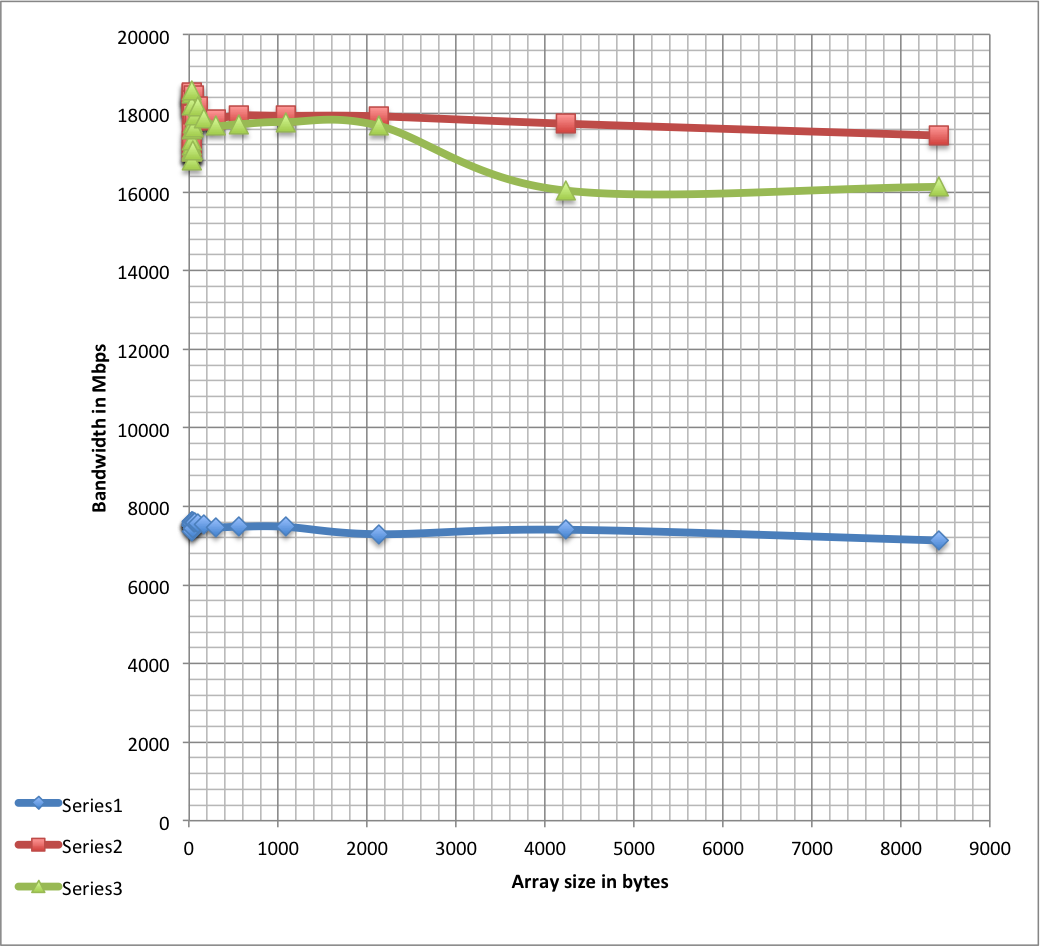
\includegraphics[width=0.8\textwidth]{graph_mem.png}
%\caption{series 1: inefficient routine; series 2: simd\_memcpy; series 3: simd\_memcpy\_cache}
%\label{fig:awesome_image}
%\end{figure}



\end{document}








% \begin{lstlisting}[label=some-code,caption=Some Code]
% public void here() {
% goes().the().code()
% }
% \end{lstlisting}








